\documentclass[10pt,a4paper,twocolumn]{article}
\newcommand{\runningtitle}{Evaporation and the baryon excess}
\newcommand{\paperfooter}{Revised exploratory study | 18 October 2026}
\usepackage[utf8]{inputenc}
\usepackage[T1]{fontenc}
\usepackage{lmodern}
\usepackage[margin=17mm,top=18mm,bottom=19mm,columnsep=6.5mm]{geometry}
\usepackage{amsmath,amssymb,array,booktabs,graphicx,xcolor,microtype}
\usepackage[authoryear,round]{natbib}
\usepackage{caption,stfloats,fancyhdr,balance}
\usepackage{multicol}
\usepackage[unicode,colorlinks=true,linkcolor=navy,citecolor=navy,urlcolor=navy]{hyperref}
\definecolor{navy}{HTML}{173B56}
\setlength{\parindent}{1em}
\setlength{\parskip}{1pt}
\raggedbottom
\clubpenalty=10000
\widowpenalty=10000
\setlength{\emergencystretch}{1.7em}
\setlength{\intextsep}{9pt}
\setlength{\textfloatsep}{11pt}
\setlength{\dbltextfloatsep}{11pt}
\setcounter{topnumber}{3}
\setcounter{dbltopnumber}{2}
\renewcommand{\topfraction}{.92}
\renewcommand{\dbltopfraction}{.95}
\renewcommand{\textfraction}{.08}
\renewcommand{\floatpagefraction}{.82}
\renewcommand{\dblfloatpagefraction}{.82}
\captionsetup{font=small,labelfont=bf,labelsep=period,skip=5pt}
\pagestyle{fancy}
\fancyhf{}
\fancyhead[L]{\footnotesize\color{navy}\runningtitle}
\fancyhead[R]{\footnotesize Andrés Germán García}
\fancyfoot[L]{\footnotesize\paperfooter}
\fancyfoot[R]{\footnotesize\thepage}
\setlength{\headheight}{13pt}
\renewcommand{\headrulewidth}{.35pt}
\newcommand{\fB}{f^{(s)}_{B\bar B}}
\newcommand{\sB}{s_{B+\bar B}}
\newcommand{\stot}{s_{\mathrm{tot}}}
\newcommand{\shad}{s_{\mathrm{had}}}
\newcommand{\sL}{s_{\mathrm{light}}}
\newcommand{\YB}{Y_{\Delta B}}
\newcommand{\doi}[1]{\href{https://doi.org/#1}{doi:#1}}
\newcommand{\fulltitle}[3]{%
\twocolumn[%
\begin{center}
{\fontsize{18}{20.5}\selectfont\bfseries\color{navy}#1\par}
\vspace{8pt}
{\normalsize Andrés Germán García\par}
{\small #2\par}
\vspace{7pt}
{\small #3\par}
\end{center}
\vspace{6pt}
\begin{minipage}{\textwidth}
\textbf{\abstractlabel.} \abstracttext
\vspace{6pt}\par
\textbf{\keywordslabel:} \keywordstext
\end{minipage}
\vspace{15pt}
]%
}


\setcitestyle{numbers,square}
\newcommand{\nb}{{n_{\bar B}}}
\newcommand{\Y}{{Y_\Delta}}
\newcommand{\sbar}{\bar s}
\newcommand{\abstractlabel}{Abstract}
\newcommand{\keywordslabel}{Keywords}
\newcommand{\abstracttext}{We quantify how thermal energy injection with no net baryon-number source changes a homogeneous expanding plasma between 50 and 30 MeV. A hypothetical population of nonrotating black holes is coupled to a thermal bath and an effective baryon-antibaryon production and annihilation equation. For an initial black-hole mass of $10^8$ g and initial black-hole-to-plasma energy-density ratios $f=0$, 0.01, 0.1, and 1, the reduced bath yields comoving plasma-entropy growth factors of 1.0000, 1.0109, 1.1093, and 2.0798. Net baryon number per entropy decreases inversely; the reduction is 51.92\% for $f=1$. With a common initial excess, the crossing $n_{\bar B}/(n_B-n_{\bar B})=1$ shifts from 38.205 to 37.974 MeV. With the initial excess adjusted to a common final yield, it instead shifts from 38.204 to 39.263 MeV. The complete PDG2025 hadron resonance gas gives 39.269 MeV for the latter $f=1$ case. A local mass scan identifies a reheating trajectory with three crossings. Separate equilibrium calculations impose charge and strangeness neutrality with vanishing net lepton numbers; these constraints are not evolved in a coupled kinetic network. A repeated execution reproduced all 36 compared CSV files. The study quantifies the consequences of specified energy deposition and boundary conditions; the final baryon yield is an input constraint, and convergence tests do not determine total physical uncertainty.}
\newcommand{\keywordstext}{baryon excess; entropy production; black-hole evaporation; pair kinetics; cosmological expansion.}
\hypersetup{pdftitle={Symmetric Evaporation and Entropy Dilution of the Baryon Excess between 50 and 30 MeV},pdfauthor={Andrés Germán García}}
\begin{document}
\fulltitle{Symmetric Evaporation and Entropy Dilution of the Baryon Excess between 50 and 30 MeV}{Independent Researcher, Mexico}{Original Spanish version: 13 October 2026 | English revision: 18 October 2026}

\section{Introduction}
The difference between baryon and antibaryon populations does not specify how many pairs coexisted at an earlier epoch. Recovering those populations requires additional relations involving temperature, composition, equilibrium or kinetics, and initial conditions. Satarov, Mishustin, and Greiner \cite{satarov} formulate production and annihilation equations for expanding systems. Yang and Rafelski \cite{yang} report a temperature of 38.2 MeV for equality between the antibaryon density and the net baryon excess under their thermal and cosmological conditions.

The companion equilibrium reconstruction \cite{garcia} evaluates fixed HRG inventories with a net-baryon-to-entropy ratio constrained by cosmological input. Five rounded density pairs from that calculation provide the initial equilibrium closure used here. A subsequent robustness calculation replaces this tabulated closure with direct sums over the complete fixed inventories.

The question addressed is how energy injection by evaporation changes plasma entropy, the normalized excess, and abundance crossings. Evaporation-driven reheating is an established mechanism \cite{haque}; the present contribution is a controlled numerical comparison of two boundary-value choices. One comparison fixes the initial excess, whereas the other adjusts it to reach the same final yield. Their distinction is essential when interpreting the direction of a crossing shift. The calculation does not fit a black-hole population or cosmological history to observations.

\section{Reference model and methods}
\subsection{Variables and initial conditions}
We adopt a spatially flat, expanding FLRW geometry with $a_i=1$ and $T_i=50$ MeV. Time $t=0$ denotes the beginning of the calculation. Define
\begin{align}
\Delta&=n_B-\nb, & \sbar&=s_{\rm pl}/k_B,\\
\Y&=\Delta/\sbar, & S_{\rm pl}&=a^3\sbar,\\
R&=\nb/\Delta, & A&=\frac{\Delta}{n_B+\nb}=\frac{1}{1+2R}.
\end{align}
$S_{\rm pl}$ is the plasma entropy, divided by $k_B$, per reference comoving volume. It does not include horizon entropy. The relative population asymmetry $A$ and the net yield $\Y$ are distinct observables of the model.

For the first reduced-bath comparison, we fix $\Delta_i=8.8765\times10^{27}$ cm$^{-3}$ and vary $f=\rho_{{\rm BH},i}/\rho_{{\rm pl},i}=0$, 0.01, 0.1, and 1. These initial black-hole abundances are assumed parameters, rather than measurements or formation fractions. The second comparison adjusts $\Delta_i$ to achieve a common final net yield.

\subsection{Thermal bath and equilibrium closure}
The reduced bath contains massless photons, electrons and positrons, three flavors of massless neutrinos and antineutrinos, massive muons, and neutral and charged pions. All bath chemical potentials vanish. The massless sector has $g_*=10.75$. For each massive species,
\begin{align}
p_j&=\frac{g_jm_j^2T^2}{2\pi^2(\hbar c)^3}
\sum_{k=1}^{64}\frac{c_{j,k}}{k^2}K_2(kx_j),\\
\rho_j&=\frac{g_jm_j^2T^2}{2\pi^2(\hbar c)^3}
\sum_{k=1}^{64}c_{j,k}\left[\frac{3K_2(kx_j)}{k^2}+\frac{x_jK_1(kx_j)}{k}\right],
\end{align}
where $x_j=m_j/T$, $c_{j,k}=1$ for bosons, and $c_{j,k}=(-1)^{k+1}$ for fermions. We add $\rho_{\rm rel}=\pi^2g_*T^4/[30(\hbar c)^3]$ and $p_{\rm rel}=\rho_{\rm rel}/3$, using $\hbar c=1.973269804\times10^{-11}$ MeV cm and $\sbar=(\rho_{\rm pl}+p_{\rm pl})/T$.

Thermodynamic functions are tabulated at 1800 temperatures between 10 and 100 MeV and interpolated with cubic splines. Initially, $\sbar_i=1.01998166\times10^{38}$ cm$^{-3}$ and $\Y_i=8.70260743\times10^{-11}$. This bath entropy is 0.1083\% below the companion HRG value, so its yield normalization differs slightly.

The equilibrium product $b_0(T)^2=n_B^{\rm eq}n_{\bar B}^{\rm eq}$ is reconstructed by PCHIP interpolation of $\log\sqrt{n_Bn_{\bar B}}$ from Table~\ref{tab:input}. This assumes an effective Boltzmann closure with $|B|=1$. Outside 37--50 MeV, $b_0$ is continued with the temperature dependence $T K_2(938.92/T)$. Reported crossings lie inside the tabulated interval; reduced-model populations at 30 MeV depend on the continuation.

\begin{table}[t]
\centering\small
\caption{Rounded equilibrium inputs from the companion reconstruction \cite{garcia}. Densities are in cm$^{-3}$ and are calculated quantities.}\label{tab:input}
\begin{tabular}{rrr}\toprule
$T$ (MeV)&$n_B$&$n_{\bar B}$\\\midrule
37&$4.4167\times10^{27}$&$1.1116\times10^{27}$\\
38.203739&$7.3454\times10^{27}$&$3.6727\times10^{27}$\\
40&$1.9166\times10^{28}$&$1.4894\times10^{28}$\\
45&$2.8323\times10^{29}$&$2.7694\times10^{29}$\\
50&$2.7261\times10^{30}$&$2.7172\times10^{30}$\\\bottomrule
\end{tabular}
\end{table}

\subsection{Evaporation and expansion}
Each black hole starts at $M_i=10^8$ g. The semiclassical approximation adopted from Ref.~\cite{cai} is
\begin{align}
\dot M&=-\alpha/M^2,\\
\alpha&=(5.34\times10^{25})(15.35)\;\mathrm{g^3\,s^{-1}},\\
\tau&=\frac{M_i^3}{3\alpha}=4.066578\times10^{-4}\;\mathrm{s}.
\end{align}
Here $\tau$ is the remaining lifetime from $M_i$. The coefficient is constant; accretion, rotation, remnants, and subsequent formation are excluded. This approximation does not resolve the quantum endpoint of evaporation.

With $m=M/M_i$, the coupled energy equations are
\begin{align}
\rho_{\rm BH}&=f\rho_{{\rm pl},i}m/a^3,\\
Q&=-f\rho_{{\rm pl},i}\dot m/a^3,\\
H^2&=\frac{8\pi G}{3c^2}(\rho_{\rm pl}+\rho_{\rm BH}),\quad H>0,\\
\dot\rho_{\rm pl}+3H(\rho_{\rm pl}+p_{\rm pl})&=Q.
\end{align}
Energy densities in the Friedmann equation are converted from MeV cm$^{-3}$ to erg cm$^{-3}$. All lost energy is deposited immediately in the bath, so $f_{\rm dep}=1$. This assumption idealizes thermalization and omits energy loss into decoupled channels. The complementary equation $\dot\rho_{\rm BH}+3H\rho_{\rm BH}=-Q$ restores the total energy balance when the two components are added.

\subsection{Baryon-antibaryon kinetics}
We integrate
\begin{equation}
\dot n_{\bar B}+3H\nb=\langle\sigma v\rangle\left[b_0^2-\nb(\nb+\Delta)\right],
\end{equation}
with the parametrization in Eq.~(9) of Satarov et al. \cite{satarov},
\begin{equation}
\langle\sigma v\rangle=\left(3.5+8.6\sqrt{T/(939\;\mathrm{MeV})}\right)\mathrm{fm^2}\,c.
\end{equation}
The code converts fm$^2$ to cm$^2$ and uses $c$ in cm s$^{-1}$. This nucleonic rate is applied effectively to the total baryonic population. The inverse term allows thermal pair production. Direct hadronic injection from Hawking cascades and a net baryon-number source are absent.

Net comoving baryon number is conserved by imposing
\begin{equation}\label{eq:net}
\Delta=\Delta_i/a^3,\qquad n_B=\nb+\Delta.
\end{equation}
The initial equilibrium state is compatible with the tabulated product and selected excess:
\begin{equation}
\nb_i=\frac{2b_0(T_i)^2}{\sqrt{\Delta_i^2+4b_0(T_i)^2}+\Delta_i}.
\end{equation}
This expression avoids cancellation. Pairs form a test sector: their evolving composition does not feed back into bath energy or entropy.

\subsection{Entropy identity and numerical method}
The balances and vanishing bath chemical potentials imply
\begin{align}
\frac{dS_{\rm pl}}{dt}&=\frac{a^3Q}{T},\\
\frac{\Y(t)}{\Y_i}&=\frac{S_{{\rm pl},i}}{S_{\rm pl}(t)},\label{eq:dil}\\
\dot Y_\Delta&=-\Y\frac{Q}{T\sbar}.
\end{align}
For $Q\geq0$ and a positive excess, $\Y$ cannot increase. Dilution follows analytically from the stated balances; integration determines its magnitude for each scenario.

SciPy's \texttt{solve\_ivp} is used with BDF. During evaporation, the independent variable is $u=1-M/M_i$, with $dt/du=3\tau(1-u)^2$, regularizing the divergent endpoint power. The evolved variables are $N=\ln a$, $T$, $z=a^3\nb/10^{30}$, and a separate estimate of $S_{\rm pl}/S_{{\rm pl},i}$. After evaporation, integration proceeds in $N$ until $T=30$ MeV.

The relative tolerance is $2\times10^{-7}$; the absolute tolerances during evaporation are $10^{-10}$, $10^{-8}$, $10^{-14}$, and $10^{-10}$ for the four variables, respectively. The $f=1$ case is repeated at a tenfold smaller relative tolerance. The maximum step is 0.008 in each independent variable, and 1201 samples are exported per trajectory. Crossing roots are found with Brent's method on the integrator's dense output by solving $z=\Delta_i/10^{30}$.

\subsection{Common-final-yield comparison}
We adopt $\Y_{\rm obj}=(6.12\times10^{-10})/7.04=8.693181818\times10^{-11}$, retaining the companion cosmological input \cite{garcia,pdg}. Applying this target at 30 MeV assumes subsequent conservation of comoving net baryon number and the entropy under consideration.

Because the pair sector does not backreact on the bath, $F(f)=S_{{\rm pl},f}/S_{{\rm pl},i}$ is independent of $\Delta_i$ within this model. We use the initial run to set
\begin{equation}\label{eq:boundary}
\Delta_i(f)=\sbar_i F(f)\Y_{\rm obj}.
\end{equation}
All four cases are reintegrated, recalculating initial equilibrium populations, kinetics, and crossings. The final common yield is an imposed boundary condition. Agreement with that target tests implementation rather than predicting the yield. The $f=1$ case is repeated with a smaller tolerance and the same $\Delta_i$, without retuning.

\section{Results for the reduced bath}
\subsection{Entropy and normalized excess}
Table~\ref{tab:results} summarizes the solutions, and Figure~\ref{fig:results} shows the trajectories. Without black holes, comoving entropy remains constant within numerical error. For $f=0.01$, 0.1, and 1, it increases by approximately 1.09\%, 10.93\%, and 107.98\%, respectively.

For $f=1$, $S_{{\rm pl},f}/S_{{\rm pl},i}=2.079842$ and $\Y_f=4.184264\times10^{-11}$, a reduction of 51.92\% from $\Y_i$. Comoving net baryon number remains fixed; dilution arises from the increasing entropy denominator.

\begin{table}[t]
\centering\small
\caption{Reduced bath with common initial excess. Entropy and yield are reported at 30 MeV; $T_\times$ is the crossing temperature along the trajectory. Digits document numerical comparisons.}\label{tab:results}
\begin{tabular}{rrrr}\toprule
$f$&$S_f/S_i$&$\Y_f$&$T_\times$ (MeV)\\\midrule
0&1.0000&$8.703\times10^{-11}$&38.205\\
0.01&1.0109&$8.608\times10^{-11}$&38.202\\
0.1&1.1093&$7.845\times10^{-11}$&38.176\\
1&2.0798&$4.184\times10^{-11}$&37.974\\\bottomrule
\end{tabular}
\end{table}

\begin{figure*}[t]
\centering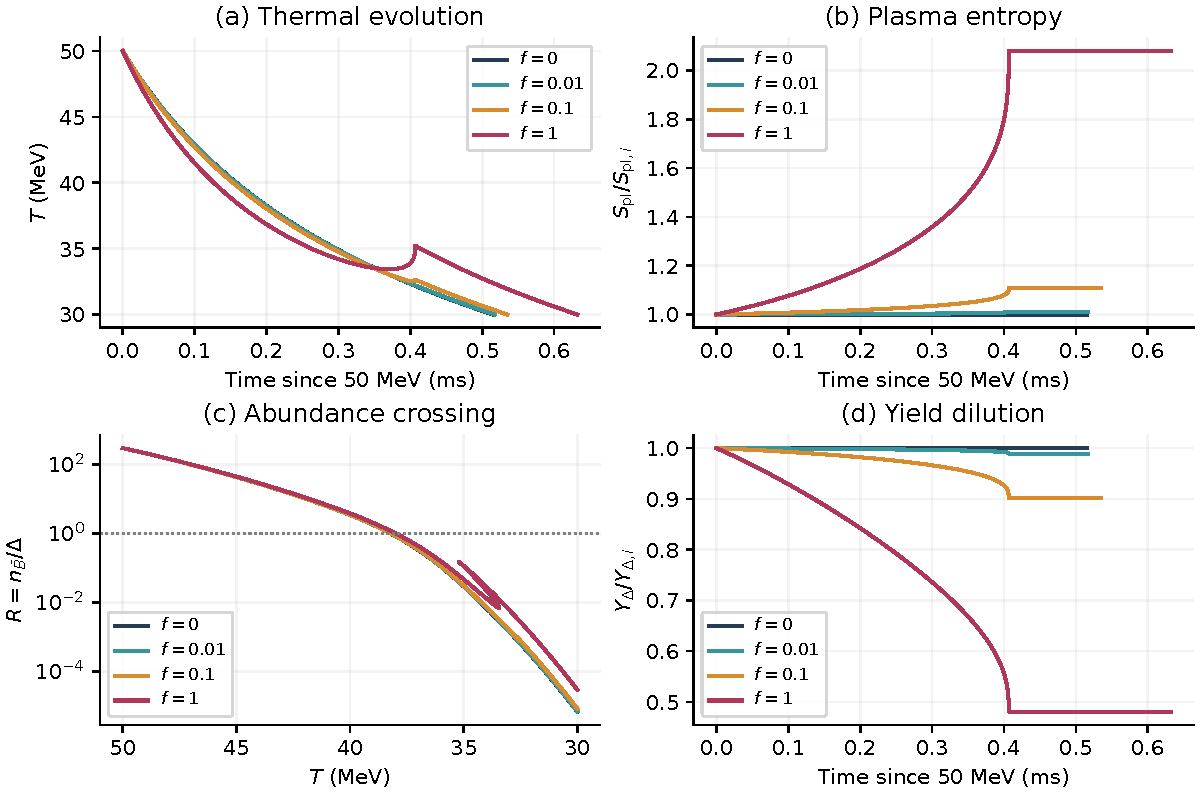
\includegraphics[width=.98\textwidth]{figures_en/initial_excess.pdf}
\caption{Calculated trajectories with common initial baryonic conditions. (a) Plasma temperature. (b) Comoving plasma entropy. (c) Antibaryon-to-net-excess ratio, with $R=1$ marked. (d) Yield relative to its initial value. The reciprocity between (b) and (d) follows from the imposed balance. Each case ends at 30 MeV at a different time.}\label{fig:results}
\end{figure*}

\subsection{Crossing and partial reheating}
The crossing shifts by approximately $-0.232$ MeV between $f=0$ and $f=1$. At $R=1$, $n_B=2\nb$ and $A=1/3$; antibaryons remain present. The criterion does not define their disappearance or chemical freeze-out.

The control yields 38.2054 MeV, close to the 38.2 MeV reference \cite{yang}. This proximity is expected from shared thermal inputs and is not an independent validation of the cosmological scenario. The bath and chemical conditions also differ between the models.

For $f=1$, the sampled temperature reaches a minimum near 33.44 MeV, then rises to 35.219 MeV at completion of evaporation before cooling to 30 MeV. Reheating is partial: none of these trajectories exceeds the initial temperature. Its details depend on the instantaneous-deposition assumption.

\subsection{Relative asymmetry and numerical checks}
All cases start at $A_i\simeq0.001631$. For $f=1$, $A_f\simeq0.999942$ at 30 MeV while $\Y$ decreases. Increasing baryon dominance in the remaining population can therefore coexist with dilution of the net yield. The conserved quantity is $a^3\Delta$, whereas the physical density $\Delta$ decreases as $a^{-3}$.

Two evaluations of the entropy balance differ by less than $8.2\times10^{-9}$ relatively. Reducing the tolerance changes $S_{{\rm pl},f}$ and $\Y_f$ by $4.2\times10^{-9}$ relatively. Exported densities are positive. Compared with the earlier sampled crossing estimates, dense-output roots shift by $1.09\times10^{-4}$ to $1.96\times10^{-4}$ MeV. For $f=1$, the dense-output root changes by $1.53\times10^{-8}$ MeV under the tighter tolerance. The largest sampled departure from instantaneous chemical equilibrium is approximately 0.68\%, near the emission endpoint. This is a property of the adopted idealization, not a transport prediction.

\subsection{Results at a common final yield}
Table~\ref{tab:normalized} gives the four reintegrations. The required initial yield rises from $8.693\times10^{-11}$ in the control to $1.808\times10^{-10}$ for $f=1$. In the latter case, $\Delta_i=1.844\times10^{28}$ cm$^{-3}$. Entropy-growth factors match those of the first comparison within numerical error.

\begin{table}[t]
\centering\small
\caption{Reduced bath with imposed $\Y_f=8.69318\times10^{-11}$. The central columns show the required initial yield and density.}\label{tab:normalized}
\setlength{\tabcolsep}{4pt}
\begin{tabular}{rrrr}\toprule
$f$&$\Y_i\;(10^{-11})$&$\Delta_i\;(10^{27}\,\mathrm{cm}^{-3})$&$T_\times$ (MeV)\\\midrule
0&8.693&8.867&38.204\\
0.01&8.788&8.964&38.219\\
0.1&9.644&9.836&38.349\\
1&18.080&18.442&39.263\\\bottomrule
\end{tabular}
\end{table}

The crossing rises by approximately 1.059 MeV between $f=0$ and $f=1$, compared with the 0.232 MeV decrease at fixed initial excess. The $f=1$ crossings differ by 1.289 MeV between protocols. These comparisons involve different initial baryonic conditions. Even the controls differ slightly because the second protocol imposes exactly $\eta/7.04$ in the reduced bath.

The relative error against the final target is below $5\times10^{-9}$ in all four runs. Repeating $f=1$ changes $\Y_f$ by $5.05\times10^{-10}$ relatively and $T_\times$ by $8.97\times10^{-8}$ MeV. Positivity and the initial equilibrium product are also verified. These checks quantify computational precision.

\begin{figure*}[t]
\centering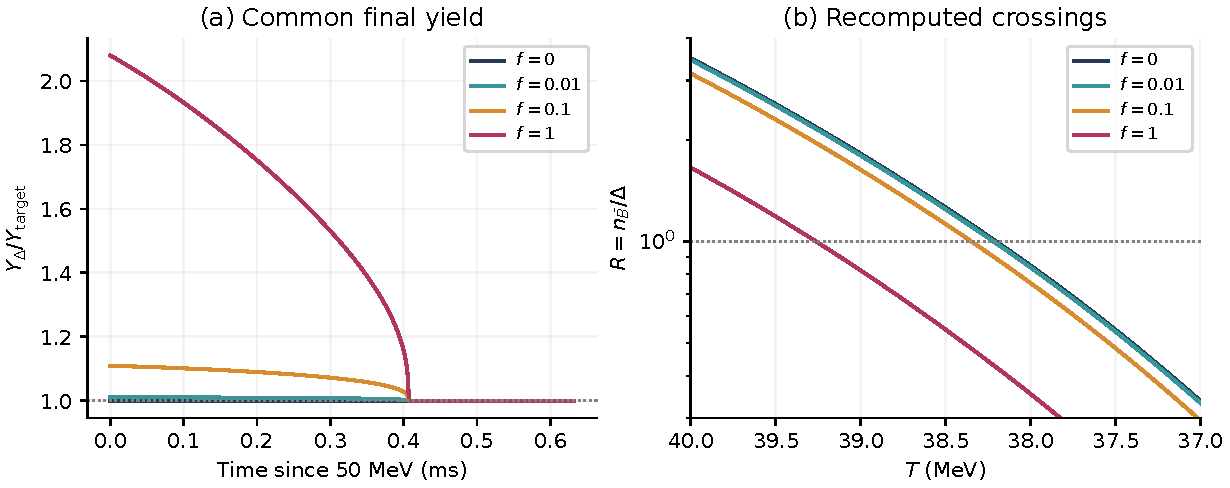
\includegraphics[width=.98\textwidth]{figures_en/final_yield.pdf}
\caption{Reintegrated scenarios with a common final yield. (a) Different initial yields reach $\Y_{\rm obj}$ by construction. (b) Enlarged crossing region: increasing $f$ requires a larger initial excess, and $R=1$ occurs at higher temperature in these cases. Initial black-hole mass and all other model assumptions are held fixed.}\label{fig:normalized}
\end{figure*}

\section{Robustness with complete inventories}
\subsection{Reproduction and thermal implementation}
The archived HRG package was recovered, and the SHA-256 hashes of the PDG2014, PDG2020, and PDG2025 Thermal-FIST lists \cite{fist} were checked against its records. The declared repository revision is \texttt{4086191e9522}; its remote copy was not independently verified in the present revision. The original calculation, including 24 checks and 1329 species-level records, was rerun. A second thermal implementation reproduces populations and excess at five temperatures in the three catalogs with a maximum relative discrepancy of $2.92\times10^{-13}$. This compares implementations sharing the same inventories.

All active inventory entries, antiparticles, and the same leptonic sector are included. Nominal masses, zero resonance widths, and the absence of interactions are retained. The Thermal-FIST C++ program is not executed; its data are evaluated with Python.

For evolution, $\rho$, $p$, and $\log b_0$ at vanishing chemical potentials are tabulated on 801 temperatures between 20 and 80 MeV using 64 Bessel terms. Scaled Bessel functions and combined mass and chemical-potential exponents avoid indeterminate products in the 128-term check. The species sums replace the five rounded inputs and nucleonic extrapolation; dense-grid splines are queried by the integrator.

The test-sector approximation remains: the bath uses equilibrium populations at zero chemical potentials and receives no feedback from kinetic composition. The product $b_0^2$ retains the effective Boltzmann closure. The following chemical checks assess selected equilibrium states, not a coupled chemical evolution.

\subsection{Equilibrium neutrality control}
We solve simultaneously for the chemical potentials associated with baryon number, electric charge, strangeness, and electron and muon lepton numbers, imposing
\begin{equation}
\Delta/\sbar=\Y_{\rm obj},\quad n_Q=n_S=n_{L_e}=n_{L_\mu}=0.
\end{equation}
We also take $n_{L_\tau}=0$, with zero tau-neutrino chemical potential and no charged tau leptons. For each species,
\begin{align}
\mu_i={}&B_i\mu_B+Q_i\mu_Q+S_i\mu_S\nonumber\\
&+L_{e,i}\mu_{L_e}+L_{\mu,i}\mu_{L_\mu}.
\end{align}
Vanishing net lepton numbers are an explicit control choice. Their potential influence on the cosmic trajectory is documented by Wygas et al. \cite{wygas}.

In the tested PDG2025 states between 30 and 50 MeV, all normalized residuals are below the acceptance threshold $10^{-7}$; the largest obtained residual is $8.32\times10^{-16}$. The equilibrium crossing remains 38.203739 MeV, differing from the nonneutral baseline by less than $10^{-8}$ MeV under these assumptions. This insensitivity is not extrapolated to other lepton asymmetries.

Relative energy and entropy corrections against the zero-potential bath are below $3.8\times10^{-9}$ and $2.5\times10^{-9}$ at the checked states. The product $n_Bn_{\bar B}/b_0^2$ differs from unity by less than $3.5\times10^{-12}$. These are local equilibrium diagnostics, not error bounds on nonequilibrium trajectories. Neutrality is not imposed dynamically in the effective pair equation.

\subsection{Reintegration and mass sensitivity}
To compare thermal backgrounds, the first protocol fixes the same initial yield $\Y_i=\Y_{\rm obj}$ and calculates $\Delta_i$ using each background's initial entropy. Within one background this also fixes the initial density across $f$. The second protocol fixes $\Y_f=\Y_{\rm obj}$. For PDG2025, $M_i=10^8$ g, and $f=1$, the latter gives $S_f/S_i=2.079958$, $\Y_i=1.808146\times10^{-10}$, and a crossing at 39.269261 MeV. Its shift from the reduced bath is $+0.006241$ MeV. The crossing range among the three catalogs is approximately 0.000152 MeV and measures inventory sensitivity.

Twelve combinations of $M_i=(0.70,0.85,1.00)\times10^8$ g and $f=0$, 0.01, 0.1, and 1 were integrated under both protocols, giving 24 trajectories. This local scan keeps complete evaporation before the 30 MeV endpoint; it is not an observationally allowed parameter region. Catalog, tolerance, and thermal-grid checks were added. Final-target relative discrepancies remain below $2\times10^{-8}$ across the scan.

\begin{table*}[t]
\centering\small
\caption{PDG2025, $f=1$, and a common final yield. All crossings are listed in time order. Times are measured from the start at 50 MeV. Instantaneous energy deposition is assumed.}\label{tab:mass}
\begin{tabular}{rrrrl}\toprule
$M_i$ ($10^8$ g)&$S_f/S_i$&$\Y_i$ ($10^{-11}$)&Crossings&Crossing temperatures (MeV)\\\midrule
0.70&1.854078&16.11784&1&38.203739\\
0.85&1.955012&16.99528&3&38.846320; 38.541989; 38.203739\\
1.00&2.079958&18.08146&1&39.269261\\\bottomrule
\end{tabular}
\end{table*}

For $M_i=0.70\times10^8$ g, evaporation ends at 45.983 MeV, before the crossing; the yield has already reached its target at $R=1$. For $M_i=0.85\times10^8$ g, $R$ first crosses downward, then upward during reheating, and finally downward after evaporation (Figure~\ref{fig:multi}). The corresponding elapsed times are 0.187886, 0.237485, and 0.301677 ms. For $10^8$ g, the common-final-yield protocol has one crossing.

The first, last, or complete crossing set must therefore be specified. Scalar crossing columns in the scan summaries identify the last crossing, while complete lists are retained. Multiple abundance crossings describe the local cooling and reheating trajectory.

\begin{figure*}[t]
\centering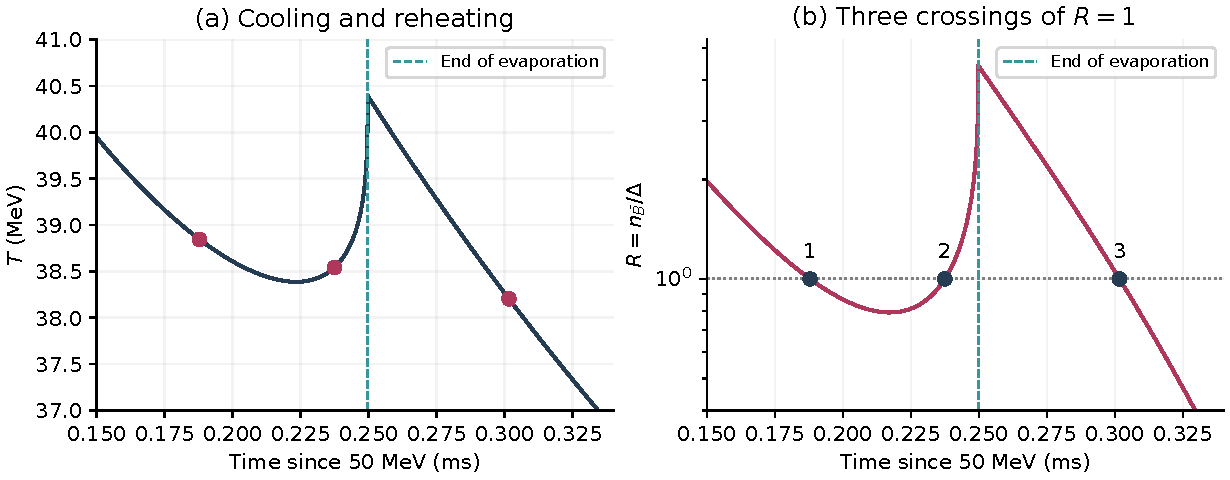
\includegraphics[width=.98\textwidth]{figures_en/multiple_crossings.pdf}
\caption{Three-crossing case with $M_i=8.5\times10^7$ g, $f=1$, the PDG2025 bath, and a common final yield. (a) Plasma temperature. (b) Crossings of $R=1$, numbered chronologically. The vertical line marks completion of evaporation. Cooling, energy injection, and thermal pair readjustment jointly determine this behavior.}\label{fig:multi}
\end{figure*}

For this case, a tenfold tolerance reduction changes crossing temperatures by less than $2.3\times10^{-8}$ MeV; doubling thermal-grid resolution changes them by less than $1.6\times10^{-8}$ MeV. All three crossings persist. For $M_i=10^8$ g and $f=1$, the crossing changes by $1.50\times10^{-8}$ MeV under the tighter tolerance and $2.77\times10^{-11}$ MeV under grid refinement. These checks address those numerical settings rather than finite-time thermalization, Hawking spectra, or nonthermal transport.

\subsection{Verification of the archived results}
For the 18 October revision, the reduced calculation, common-final-yield calculation, full-inventory scan, thermal-source comparison, and multiple-crossing verification were executed again. All 36 compared CSV files, containing 38\,496 data rows, matched the archived versions byte for byte. The companion HRG reproduction contributed a further five matching CSV files. Logs and a file-by-file comparison record are included in the shared audit folder. The additional direct momentum-integral check belongs to the companion equilibrium study; it is not an independent reimplementation of the full evaporation dynamics.

\section{Discussion}
\subsection{What the calculation establishes}
The model quantifies dilution of a conserved comoving excess when entropy is injected. Equation~\eqref{eq:dil} fixes the sign of the yield change, while bath and expansion dynamics determine its magnitude. The numerical results distinguish this analytic identity from the computed entropy-growth factors, crossing shifts, and multiplicity.

The distinction between $A$ and $\Y$ is essential: pair depletion increases baryon dominance without generating net baryon number. Studying net generation would require an independently justified source in $\dot\Delta+3H\Delta=Q_{\Delta B}$, which is absent here.

\subsection{Boundary conditions and cosmological normalization}
The companion reconstruction assumes an adiabatic connection between early and present net yields. Entropy injection changes that connection. At fixed initial excess, different $f$ values lead to different final yields. At fixed final yield, different initial excesses are required. Along the latter trajectories,
\begin{equation}
\Y(t)=\Y_{\rm obj}\frac{S_{{\rm pl},f}}{S_{\rm pl}(t)}.
\end{equation}
Before injection ends, the yield must exceed its target. In the calculated cases, this normalization moves the crossing to higher temperatures even though entropy dilutes the yield along each trajectory. A crossing shift must always be associated with its comparison protocol.

Adjusting the initial excess does not explain its origin. Different initial conditions and entropy injections can reach the same final yield, so that yield alone cannot identify $f$ or establish that the hypothetical black-hole population existed.

\subsection{Physical limitations and next extension}
The kinetic equation uses an effective nucleonic rate for all baryons and does not evolve electric, strangeness, and lepton balances as a coupled network. Those balances are solved only in separate equilibrium controls. Complete inventories improve the thermal closure but do not include interactions, resonance widths, or total physical uncertainty.

The assumed mass and abundance are not linked to a formation history. Energy injection is homogeneous and instantly thermalized; spectra, cascades, a mass distribution, and observational population constraints are not calculated. Kinetic pair composition does not backreact on the bath. Entropy accounting is restricted to the modeled plasma. The expanding branch and 50--30 MeV interval also do not describe contraction, a bounce, or subsequent cosmic evolution.

A direct next extension is to replace instantaneous deposition with a specified thermalization model and assess whether the three crossings persist. A coupled chemical network would then test the charge-balance approximation along the evolving trajectory. These physical extensions are distinct from further refinement of already converged numerical settings.

\section{Conclusions}
Under the stated assumptions, evaporation increases comoving plasma entropy and dilutes net baryon number per entropy while preserving comoving net baryon number. For the reduced bath at $M_i=10^8$ g and $f=1$, entropy grows by a factor of 2.0798 and the yield falls by 51.92\%. The crossing is 37.974 MeV with common initial excess and 39.263 MeV with a common final yield.

The complete PDG2025 inventory gives 39.269 MeV for the latter case. A local mass scan yields three abundance crossings for $M_i=8.5\times10^7$ g and $f=1$; their persistence under tolerance and grid checks establishes this behavior within the numerical model. Crossing temperatures are conditional on the injection history and boundary conditions rather than universal scales.

The reproduced calculations provide a traceable comparison of equilibrium inputs, entropy injection, and pair kinetics under specified deposition and chemical approximations. They do not infer the origin of the asymmetry or establish the assumed black-hole population observationally.

\balance
\section*{Data, code, and reproducibility}
The source package includes \texttt{simular.py}, \texttt{ajustar\_exceso\_final.py}, the \texttt{robustez\_hrg} calculations, fixed inventories and licenses, CSV and JSON outputs, and an English figure-generation script. The shared audit folder retains execution logs, comparisons, and additional equilibrium checks. Runs used Linux, Python 3.12.14, NumPy 2.3.5, SciPy 1.17.0, and Matplotlib 3.10.8. Windows instructions are retained without claiming execution on that platform. The English revision changes presentation and verification reporting; the physical parameters and numerical results are retained.

\section*{Assistance in preparation}
Artificial intelligence assistance was used for code review, execution, translation, editing, and layout. The described calculations were executed and their outputs retained. Scientific interpretation and publication decisions remain the author's responsibility.

\begin{thebibliography}{9}\small
\bibitem{satarov} L. M. Satarov, I. N. Mishustin, and W. Greiner (2013). Evolution of antibaryon abundances in the early Universe and in heavy-ion collisions. \textit{Physical Review C} \textbf{88}, 024908. \doi{10.1103/PhysRevC.88.024908}.
\bibitem{yang} C. T. Yang and J. Rafelski (2022). Cosmological strangeness abundance. \textit{Physics Letters B} \textbf{827}, 136944. \doi{10.1016/j.physletb.2022.136944}. Section 3 and Figure 3.
\bibitem{garcia} A. G. García (2026). \textit{Baryon-Antibaryon Reconstruction at 50 MeV: Rest Masses and Cosmological Abundances}. Companion manuscript, original version of 9 October 2026, English revision of 18 October 2026. Included in the accompanying package; external peer review is not claimed.
\bibitem{haque} M. R. Haque, E. Kpatcha, D. Maity, and Y. Mambrini (2023). Primordial Black Hole Reheating. \href{https://arxiv.org/abs/2305.10518}{arXiv:2305.10518}. Context for reheating; its inflationary scenario is not reproduced here.
\bibitem{cai} Y.-F. Cai, C. Chen, Q. Ding, and Y. Wang (2022). Ultrahigh-energy gamma rays and gravitational waves from primordial exotic stellar bubbles. \textit{European Physical Journal C}. \doi{10.1140/epjc/s10052-022-10395-w}; \href{https://arxiv.org/abs/2105.11481}{arXiv:2105.11481}, Appendix B, Eqs.~(B3)--(B4). Only the mass-loss parametrization is used.
\bibitem{fist} V. Vovchenko and H. Stoecker (2019). Thermal-FIST: A package for heavy-ion collisions and hadronic equation of state. \textit{Computer Physics Communications} \textbf{244}, 295--310. \doi{10.1016/j.cpc.2019.06.024}. Fixed catalog files and hashes are included in the supplement.
\bibitem{wygas} M. M. Wygas, I. M. Oldengott, D. B\"odeker, and D. J. Schwarz (2018). Cosmic QCD Epoch at Nonvanishing Lepton Asymmetry. \textit{Physical Review Letters} \textbf{121}, 201302. \doi{10.1103/PhysRevLett.121.201302}. Context for lepton-number assumptions; its QCD calculation is not reproduced.
\bibitem{pdg} B. D. Fields, P. Molaro, and S. Sarkar (2025). Big Bang nucleosynthesis. \textit{Review of Particle Physics: 2025 update}, Eq.~24.8. \href{https://pdg.lbl.gov/2025/reviews/rpp2025-rev-bbang-nucleosynthesis.pdf}{PDG review}.
\end{thebibliography}
\end{document}
